% % Para el tipo de documento
%\documentclass{article} % artículo: documentos cortos
\documentclass[a4paper, 12pt]{article} % book: estilo libro. Documentos largos con capítulos
% Dependiendo del tipo de documento tiene una estructura u otra

% Para idioma Español
\usepackage[utf8]{inputenc} % uso directo y libre de los caracteres acentuados
\usepackage[english]{babel}
\usepackage[T1]{fontenc} % para seleccionar luego del pdf y mantener los acentos

% Para letra helvetica
\usepackage[scaled]{helvet}
\renewcommand\familydefault{\sfdefault}

\usepackage{seqsplit}
\usepackage{tabularx}
\usepackage{longtable}
\usepackage{adjustbox}
\usepackage{float}

% Para los fondos del documento
\usepackage{eso-pic}
\usepackage{xcolor} \definecolor{letras_blancas}{RGB}{255,255,255}
\usepackage{sectsty}
\sectionfont{\color[RGB]{0, 105, 166}}  % sets colour of sections
\subsectionfont{\color[RGB]{0, 105, 166}}  % sets colour of sections
\subsubsectionfont{\color[RGB]{0, 105, 166}}  % sets colour of sections

% Para el color gris de las letras
\makeatletter
\newcommand{\globalcolor}{%
  \color[RGB]{62, 67, 61}\global\let\default@color\current@color
}
\makeatother
\AtBeginDocument{\globalcolor}
% Fin configuración color letras

\usepackage[absolute,overlay]{textpos}

% Para la separación correcta de las palabras
\usepackage{hyphenat}
\hyphenation{mate-máti-cas recu-perar}

% Para los gráficos
\usepackage{graphicx}
\usepackage[inkscapeformat=png]{svg}
\graphicspath{ {./images} } % para indicarle que las imágenes se encuentran en la carpeta "images"

% Para hacer el documento con diferentes ficheros .tex
\usepackage{subfiles}

% Para las referencias
\usepackage{hyperref}
\hypersetup{
	colorlinks=true,
	linkcolor=black,
	filecolor=magenta,
	urlcolor=black,
	bookmarks=true,
  citecolor=black,
}
% Para la bibliografía
\usepackage{biblatex} %Imports biblatex package
\addbibresource{referencias.bib}

% Para no poner \noindent{} en cada párrafo
\setlength{\parindent}{0pt}

% Para introducir código
\usepackage{listings}
\usepackage{float}
\setcounter{tocdepth}{2} % niveles del índice

\begin{document}

% Portada e índice
\pagenumbering{gobble} % Sin numeración
%\sffamily % Letra sin serif

% Inicio Portada
\AddToShipoutPictureBG*{
\includegraphics[width=\paperwidth,height=\paperheight]{fondos/fondo_portada.jpg}}
\begin{textblock*}{15cm}(4.5cm,23cm)
    \huge{\textcolor{letras_blancas}{\textbf{TITLE}}}
\end{textblock*}
\begin{textblock*}{15cm}(12cm,28cm)
    \large{\textcolor{letras_blancas}{\textbf{AUTHOR}}}
\end{textblock*}
\mbox{}

\newpage
% Fin Portada

% Inicio Portada Sección Índice
\mbox{}
\AddToShipoutPictureBG*{
\includegraphics[width=\paperwidth,height=\paperheight]{fondos/fondo_secciones.png}}
\begin{textblock*}{15cm}(2cm,14cm)
    \huge{\textcolor{letras_blancas}{\textbf{Contents}}}
\end{textblock*}

\newpage
% Fin Portada Sección Índice

% Índice
\AddToShipoutPictureBG{
\includegraphics[width=\paperwidth,height=\paperheight]{fondos/fondo_normal.jpg}}
\tableofcontents

\clearpage
% Fin índice


% ---------------------------- Contenido ------------------------
% Inicio Portada Sección
\ClearShipoutPictureBG
\mbox{}
\AddToShipoutPictureBG*{
\includegraphics[width=\paperwidth,height=\paperheight]{fondos/fondo_secciones.png}}
\begin{textblock*}{15cm}(2cm,14cm)
    \huge{\textcolor{letras_blancas}{\textbf{Report}}}
\end{textblock*}
\newpage
% Fin Portada Sección
\newlength\mylength
\newcolumntype{C}[1]{>{\centering\arraybackslash}p{#1}}
%\newcommand{\hash}[1]{{\ttfamily\seqsplit{#1}}}

\renewcommand{\seqinsert}{\ifmmode\allowbreak\else\-\fi}
\newcommand{\wrap}[1]{\seqinsert{\seqsplit{#1}}}

% ------------------------------------- CONTENIDO ------------------------------------
\AddToShipoutPictureBG{
\includegraphics[width=\paperwidth,height=\paperheight]{fondos/fondo_normal.jpg}}

\section{Description}

DESCRIPTION

\section{APT Groups}

APT Groups associated with the provided intelligence:

GROUPS

\section{MITRE tactics, techniques and procedures}

TTP

\section{Indicators of compromise}

IOCS

\section{MITRE Kill Chain}

KILLCHAIN

\clearpage
% ------------------------------------- FIN CONTENIDO --------------------------------

% ---------------------------- Fin Contenido --------------------

% Referencias
%% Inicio Portada Sección
\ClearShipoutPictureBG
\mbox{}
\AddToShipoutPictureBG*{
\includegraphics[width=\paperwidth,height=\paperheight]{fondos/fondo_secciones.png}}
\begin{textblock*}{15cm}(3cm,14cm)
    \huge{\textcolor{letras_blancas}{\textbf{Referencias}}}
\end{textblock*}
\newpage
% Fin Portada Sección

% ------------------------------------- CONTENIDO ------------------------------------
\AddToShipoutPictureBG{
\includegraphics[width=\paperwidth,height=\paperheight]{fondos/fondo_normal.jpg}}

\printbibliography[heading=bibintoc]

\clearpage
% ------------------------------------- FIN CONTENIDO --------------------------------


% Portada final
% Inicio Portada final
\newpage
\ClearShipoutPictureBG
\AddToShipoutPictureBG{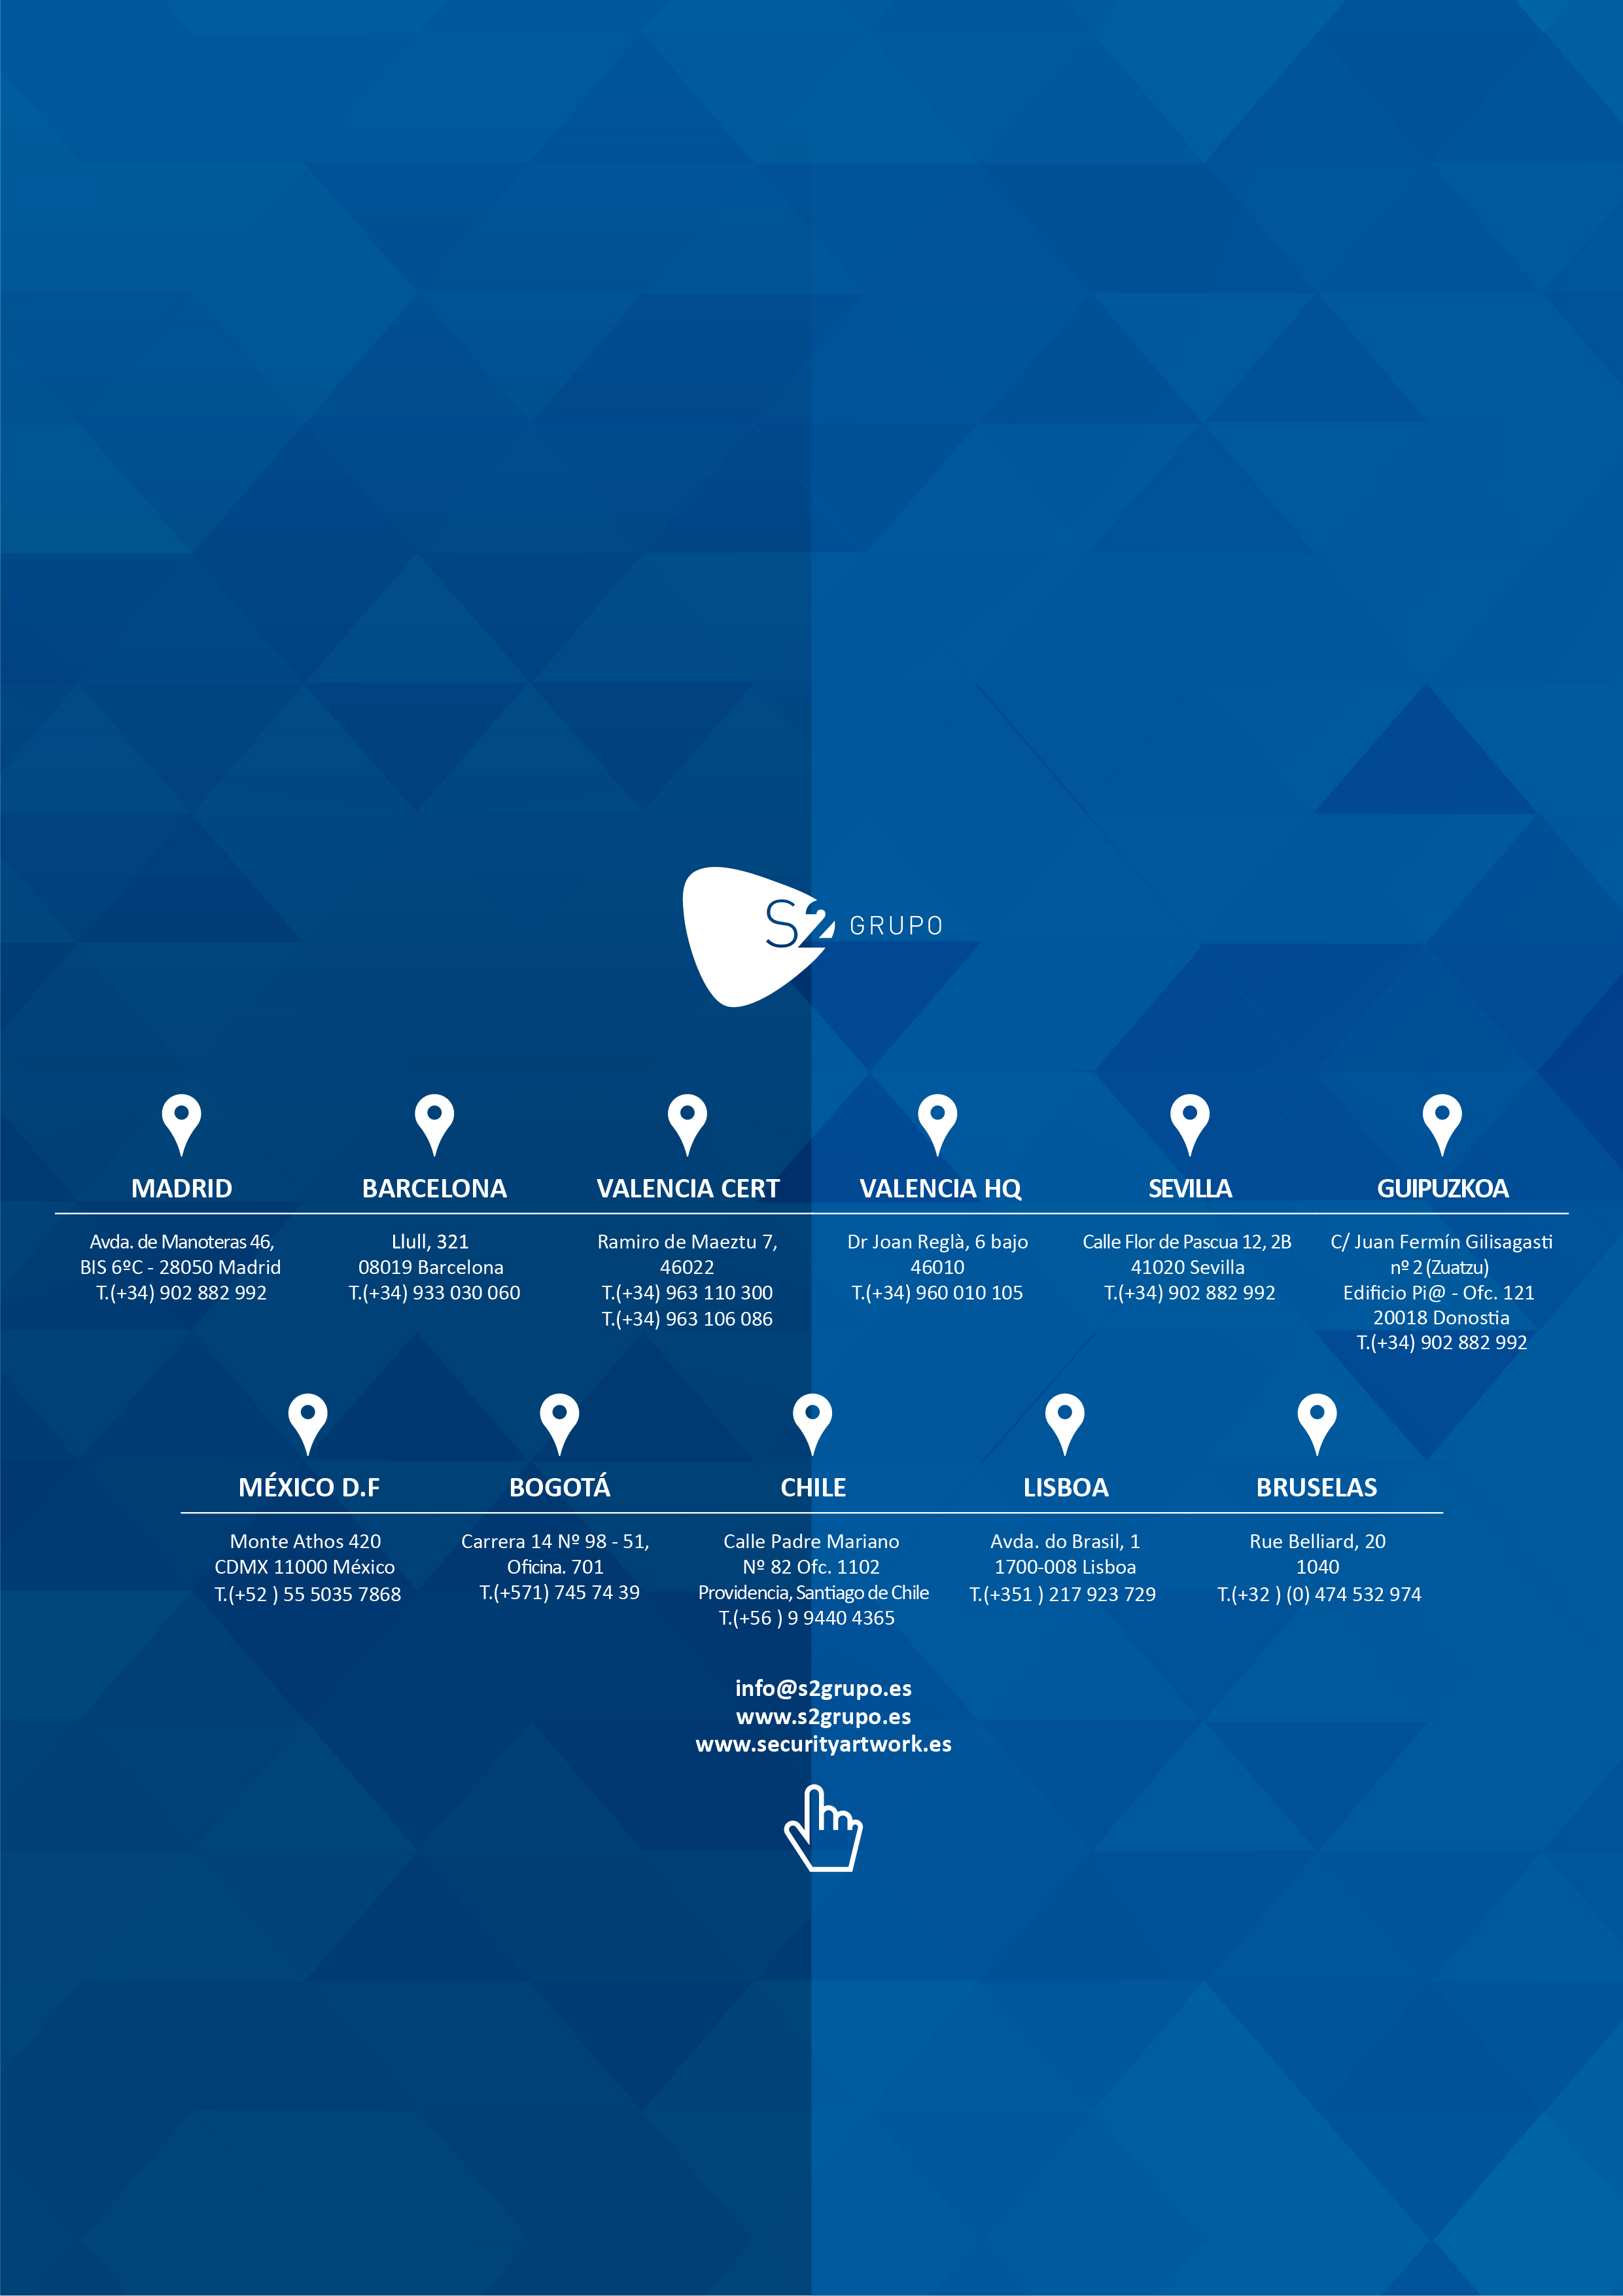
\includegraphics[width=\paperwidth,height=\paperheight]{fondos/fondo_ultima_pag.jpg}}
\mbox{}
% Fin Portada final



\end{document}
